\section{Theorie}
\label{sec:theory}
In diesem Protkoll wird das Driftverhalten von Ladungsträgern in einem Silizium-Halbleiter mithilfe der Transient-Current-Technik analysiert. Dabei wird zunächst die Transient-Current-Technik in dem \autoref{sec:tct} erläutert. Desweiteren wird in dem \autoref{sec:semi} erklärt wie ein Silizium-Halbleiter-Detektor funktioniert und daraufhin in dem \autoref{sec:drift} wird die 
\subsection{Transient-Current-Technik}
\label{sec:tct}
\begin{figure}[h]
\centering
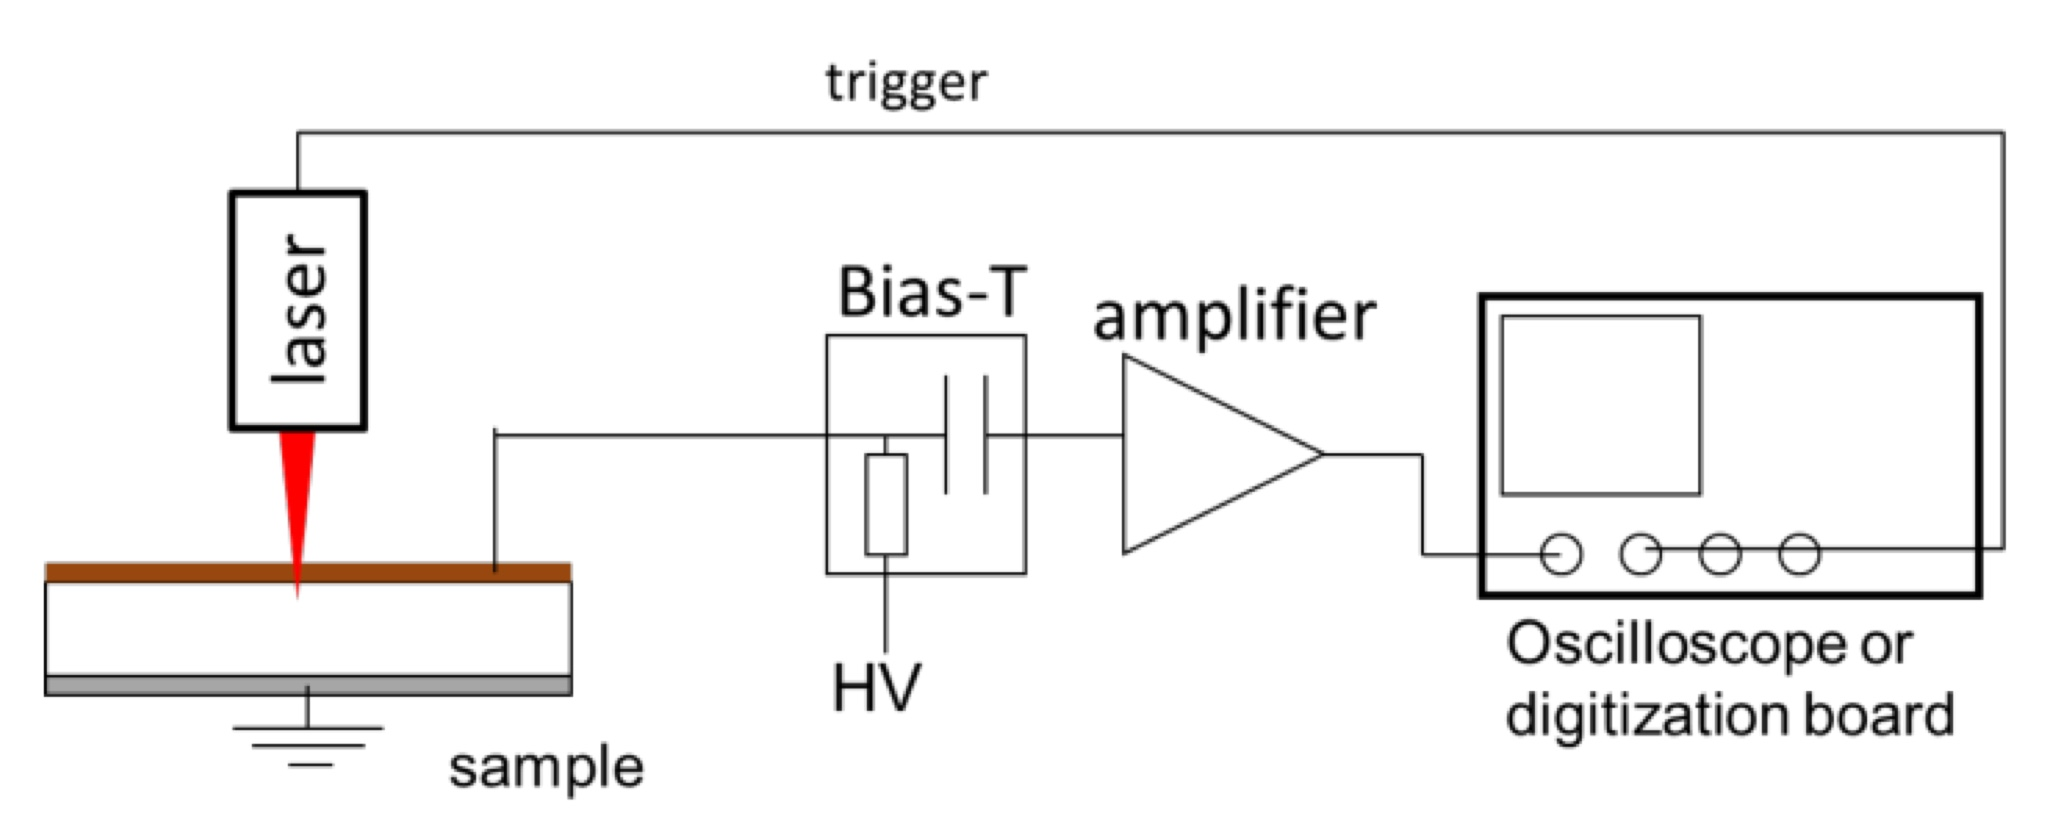
\includegraphics[width=\textwidth]{content/Figures/tct_setup.jpg}
\caption{Der schematische Versuchsaufbau der Transient-Current-Technik (TCT) \cite{Anleitung}.}
\label{fig:tct_setup}
\end{figure}
\subsection{Silizium-Halbleiter}
\label{sec:semi}
\subsection{Driftverhalten von Ladungsträgern}
\label{sec:drift}